% !TEX TS-program = lualatex
\documentclass[tikz, border=2mm, multi=forest]{standalone}

% Hỗ trợ Font Tiếng Việt cho LuaLaTeX
\usepackage{fontspec}
\IfFontExistsTF{Times New Roman}{
  \setmainfont{Times New Roman}
}{
  \setmainfont{Liberation Serif}
}
% Xử lý font cho các đoạn code \texttt
\IfFontExistsTF{Courier New}{
  \setmonofont{Courier New}[Scale=MatchLowercase]
}{}

\usepackage{forest}
\usetikzlibrary{shapes.geometric, arrows.meta, positioning, fit, backgrounds, calc, trees}

\begin{document}

% =======================================================
% === CÁC SƠ ĐỒ TỪ 03-gameEngineering.tex (Trang 26 đến 50) ===
% =======================================================

% Sơ đồ 26: Thành phần Story
\begin{tikzpicture}[
  comp/.style={rectangle,draw=blue!80,fill=blue!8,rounded corners=3pt,
               minimum width=2.9cm,minimum height=0.65cm,align=center,font=\small},
  ext/.style={rectangle,draw=gray!60,fill=gray!8,rounded corners=2pt,
              minimum width=2.4cm,minimum height=0.6cm,align=center,font=\scriptsize},
  iface/.style={-{Stealth[length=4pt]},thick},
  use/.style={-{Stealth[length=4pt]},dashed,gray}
]
  \node[comp,fill=green!15,draw=green!80] (main) at (0,0) {\texttt{Tệp\_Chính}};
  \node[comp] (entry)  at (4.5,0)   {\texttt{ChayPhanHeCotTruyen()}};
  \node[comp] (sync)   at (4.5,-1.5){\texttt{DongBoTuGist()}};
  \node[comp] (apply)  at (4.5,-3.0){\texttt{ApDungDuLieuChuong()}};
  \node[comp] (db)     at (4.5,-4.4){\texttt{TangCSDLCotTruyen()}};
  \node[comp] (psc)    at (8.8,-1.5){\texttt{KiemTraDKSauDongBo()}};
  \node[comp] (loop)   at (0,-1.5)  {\texttt{VongLapHoiThoai()}};
  \node[comp] (render) at (0,-3.0)  {\texttt{VeTrangHoiThoai()}};
  \node[ext]  (gist)  at (8.8,0)    {Máy chủ Gist\\(JSON)};
  \node[ext]  (sqlite)at (4.5,-5.8) {CSDL Cục bộ\\\texttt{CSDL\_MacDinh}};
  \node[ext]  (svg)   at (0,-4.4)   {Bộ vẽ ảnh\\Vector};
  \node[ext]  (http)  at (8.8,-4.4) {Thư viện HTTP};

  \draw[iface](main)--(entry)  node[above,font=\tiny,midway]{maTruyen, maChuong};
  \draw[iface](entry)--(sync); \draw[iface](entry)--(loop);
  \draw[iface](sync)--(apply); \draw[iface](apply)--(db);
  \draw[iface](db)--(sqlite);  \draw[iface](loop)--(render);
  \draw[use]  (render)--(svg); \draw[iface](sync)--(psc);
  \draw[use]  (sync.east)to[bend left=15]node[above,font=\tiny]{\texttt{TaiHTTPDongBo()}}(gist.south);
  \draw[use]  (sync)--(http);
\end{tikzpicture}

% Sơ đồ 27: Khởi tạo Vector
\begin{tikzpicture}[node distance=0.5cm, b/.style={rectangle,draw=blue!80,fill=blue!8,text width=2.8cm,align=center,font=\scriptsize,rounded corners=2pt,minimum height=0.6cm}]
  \node[b](a){Kiểm tra cờ\\bộ nhớ đệm};
  \node[b,right=0.6cm of a](b){Phân tích SVG\\Tính tỷ lệ};
  \node[b,right=0.6cm of b](c){Quét điểm ảnh\\$\rightarrow$ Mảng Pixel};
  \node[b,right=0.6cm of c](d){Tạo Bề mặt\\$\rightarrow$ Vật liệu};
  \node[b,right=0.6cm of d](e){Lưu vào\\Bien\_AnhVector};
  \foreach \x/\y in {a/b,b/c,c/d,d/e}{\draw[-{Stealth[length=4pt]},thick,blue!80](\x)--(\y);}
  \draw[-{Stealth[length=4pt]},thick,green!80,bend right=30](a.south)to node[below,font=\tiny]{Đã lưu $\rightarrow$ Bỏ qua}(e.south);
\end{tikzpicture}

% Sơ đồ 28: Thuật toán SHA
\begin{tikzpicture}[
  proc/.style={rectangle,draw=blue!80,fill=blue!8,rounded corners=2pt, minimum width=4.2cm,minimum height=0.55cm,align=center,font=\scriptsize},
  dec/.style={diamond,draw=orange!80,fill=orange!8, aspect=2.8,align=center,font=\scriptsize},
  term/.style={rectangle,rounded corners=3pt,draw=gray!60,fill=gray!10, minimum width=2.8cm,minimum height=0.5cm,align=center,font=\scriptsize},
  wterm/.style={rectangle,rounded corners=3pt,draw=green!80,fill=green!10, minimum width=2.8cm,minimum height=0.5cm,align=center,font=\scriptsize},
  arr/.style={-{Stealth[length=4pt]},thick}
]
  \node[proc](p0) at (0,0)    {\texttt{TaiHTTPDongBo(URL\_MAY\_CHU)}};
  \node[dec] (d0) at (0,-1.3) {Dữ liệu\\trống?};
  \node[term](off)at (4.5,-1.3){\texttt{TRANG\_THAI\_NGOAI\_TUYEN} $\rightarrow$ Thoát};
  \node[proc](p1) at (0,-2.6) {Phân tích JSON $\rightarrow$ \texttt{PhienBan[MoiNhat]}};
  \node[proc](p2) at (0,-3.7) {Duyệt từng chương: Lấy Mã băm cũ so với mới};
  \node[dec] (d1) at (0,-5.0) {Mã băm\\trùng khớp?};
  \node[term](sk) at (4.5,-5.0){Bỏ qua $\rightarrow$ Chương tiếp theo};
  \node[proc](p3) at (0,-6.3) {\texttt{TaiHTTPDongBo(URL\_Chuong)} $\rightarrow$ Dữ liệu JSON};
  \node[proc](p4) at (0,-7.4) {\texttt{ApDungDuLieuChuong(CSDL, DuLieu, maChuong)}};
  \node[proc](p5) at (0,-8.5) {\texttt{LuuMaBamMoi()}; (Cập nhật tệp ảo nếu trên Web)};
  \node[wterm](dn)at (0,-9.6) {\texttt{TRANG\_THAI\_HOAN\_TAT}};
  \draw[arr](p0)--(d0);
  \draw[arr](d0)--node[above,font=\tiny]{Có}(off);
  \draw[arr](d0)--node[left,font=\tiny]{Không}(p1);
  \draw[arr](p1)--(p2); \draw[arr](p2)--(d1);
  \draw[arr](d1)--node[above,font=\tiny]{Có}(sk);
  \draw[arr](d1)--node[left,font=\tiny]{Không}(p3);
  \draw[arr](p3)--(p4); \draw[arr](p4)--(p5); \draw[arr](p5)--(dn);
  \draw[arr,gray,dashed](sk.east) -- ++(0.6,0) |- node[pos=0.25,right,font=\tiny]{Chương kế} (p2.east);
\end{tikzpicture}

% Sơ đồ 29: Cỗ máy Trạng thái Hội thoại
\begin{tikzpicture}[node distance=1.7cm, st/.style={circle,draw=blue!80,fill=blue!8,font=\scriptsize, minimum size=1.4cm,align=center}]
  \node[st](init){KHỞI TẠO\\Tải\\lựa chọn[0]};
  \node[st,right=of init](wait){CHỜ ĐỢI\\Vẽ màn hình\\+Bắt sự kiện};
  \node[st,right=of wait](adv) {TIẾN LÊN\\Lấy mã\\Nút kế};
  \node[st,right=of adv] (chk) {KIỂM TRA\\Tải lựa chọn\\mới};
  \node[st,below=1.1cm of adv,draw=green!80,fill=green!8](end){KẾT THÚC\\Thoát hàm};
  
  \draw[-{Stealth[length=4pt]},thick,blue!80](init)--(wait);
  \draw[-{Stealth[length=4pt]},thick,blue!80](wait)--node[above, align=center, font=\tiny]{Xác nhận\\hoặc Nhấp chuột}(adv);
  \draw[-{Stealth[length=4pt]},thick,blue!80](adv)--(chk);
  \draw[-{Stealth[length=4pt]},thick,blue!80] (chk.north) to[out=145, in=35] node[above,font=\tiny]{Gán Chỉ số mới} (wait.north);
  \draw[-{Stealth[length=4pt]},thick,green!80](adv)--node[right,font=\tiny]{\texttt{maNutKe=0}}(end);
  \draw[-{Stealth[length=4pt]},thick,green!80,dashed](wait.south)to[bend right=15] node[below,font=\tiny]{Phím Thoát/Bỏ qua}(end.west);
  \draw[-{Stealth[length=4pt]},thick,blue!80,dashed](wait.north)to[bend left=20] node[above,font=\tiny]{Phím Tab $\rightarrow$ Đổi Lựa chọn}(wait.north east);
\end{tikzpicture}

% Sơ đồ 30: Sơ đồ Lớp (Thực thể Cốt truyện)
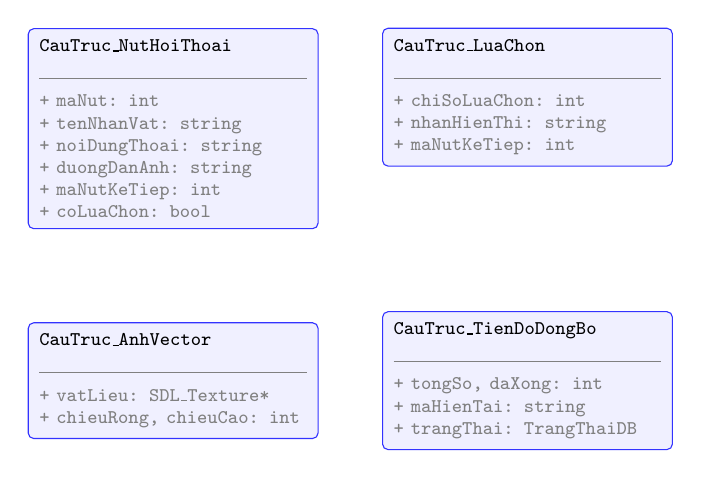
\begin{tikzpicture}[class/.style={rectangle, draw=blue!80, fill=blue!6, rounded corners=2pt, align=left, font=\scriptsize\ttfamily, inner sep=4pt}]
  \node[class, text width=3.4cm] (dn) at (0,0) {
    \textbf{CauTruc\_NutHoiThoai}\\[2pt]
    \color{gray}\rule{\linewidth}{0.4pt}\\[2pt]
    + maNut: int\\
    + tenNhanVat: string\\
    + noiDungThoai: string\\
    + duongDanAnh: string\\
    + maNutKeTiep: int\\
    + coLuaChon: bool
  };
  \node[class, text width=3.4cm] (dc) at (4.5, 0.4) {
    \textbf{CauTruc\_LuaChon}\\[2pt]
    \color{gray}\rule{\linewidth}{0.4pt}\\[2pt]
    + chiSoLuaChon: int\\
    + nhanHienThi: string\\
    + maNutKeTiep: int
  };
  \node[class, text width=3.4cm] (svg) at (0, -3.2) {
    \textbf{CauTruc\_AnhVector}\\[2pt]
    \color{gray}\rule{\linewidth}{0.4pt}\\[2pt]
    + vatLieu: SDL\_Texture*\\
    + chieuRong, chieuCao: int
  };
  \node[class, text width=3.4cm] (sp) at (4.5, -3.2) {
    \textbf{CauTruc\_TienDoDongBo}\\[2pt]
    \color{gray}\rule{\linewidth}{0.4pt}\\[2pt]
    + tongSo, daXong: int\\
    + maHienTai: string\\
    + trangThai: TrangThaiDB
  };
\end{tikzpicture}

% Sơ đồ 31: ERD Cốt truyện
\begin{tikzpicture}[
  ent/.style={rectangle,draw=blue!80,fill=blue!6,rounded corners=2pt, align=left,font=\scriptsize,inner sep=5pt,minimum width=3.4cm},
  rw/.style={rectangle,draw=green!80,fill=green!6,rounded corners=2pt, align=left,font=\scriptsize,inner sep=5pt,minimum width=3.4cm},
  rel/.style={-{Stealth[length=4pt]},thick,blue!70},
  wrrel/.style={-{Stealth[length=4pt]},thick,green!80},
  lbl/.style={font=\tiny,fill=white,inner sep=1pt}
]
  \node[ent](sd) at (0,0) {
    \textbf{DuLieu\_Chung}\ \textit{\tiny(Chỉ đọc)}\\[1pt]
    \underline{maTruyen, maChuong}\\
    tenTruyen, tenChuong\\
    nguongDiem, nguongTocDo\\
    dieuKienMoKhoa (CSV)
  };
  \node[ent](dlg) at (6,1.4) {
    \textbf{HoiThoai\_Chung}\ \textit{\tiny(Chỉ đọc)}\\[1pt]
    \underline{maTruyen, maChuong, maNut}\\
    nguoiNoi, noiDung\\
    anhMinhHoa\\
    maNutKe, coLuaChon
  };
  \node[ent](cho) at (6,-1.8) {
    \textbf{LuaChon\_Chung}\ \textit{\tiny(Chỉ đọc)}\\[1pt]
    \underline{maTruyen, maChuong,}\\
    \underline{maNut, chiSoLuaChon}\\
    nhanHienThi, maNutKe
  };
  \node[rw](meta) at (0,-3.6) {
    \textbf{SieuDuLieu\_Chung}\ \textit{\tiny(Ghi bởi hệ thống)}\\[1pt]
    \underline{maChuong} \textit{\tiny(VD: ''c001'')}\\
    maBamSHA, thoiGianCapNhat\\
    url\_MayChu
  };
  \node[rw](us) at (6,-3.8) {
    \textbf{TienDo\_NguoiDung}\ \textit{\tiny(Ghi bởi hệ thống)}\\[1pt]
    \underline{maNguoiDung, maTruyen, maChuong}\\
    daKichHoat, daChon\\
    diemCaoNhat, tocDoCaoNhat
  };
  \draw[rel](sd.north east)to[bend left=10] node[lbl,pos=0.3]{1}node[lbl,pos=0.75]{N}(dlg.west);
  \draw[rel](dlg.south)--node[lbl,left,pos=0.4]{1}node[lbl,pos=0.85]{N}(cho.north);
  \draw[rel](sd.east)to[bend right=8] node[lbl,below,pos=0.3]{1}node[lbl,pos=0.78]{N}(cho.west);
  \draw[wrrel,dashed](meta.east)-- node[lbl,above,pos=0.45]{maChuong $\leftrightarrow$ maChuong}(sd.south);
  \draw[wrrel](sd.east)to[bend left=8] node[lbl,pos=0.3]{1}node[lbl,pos=0.78]{0..1/User}(us.west);
\end{tikzpicture}

% Sơ đồ 32: DFD Cốt truyện
\begin{tikzpicture}[
  proc/.style={rectangle,draw=blue!80,fill=blue!8,rounded corners=2pt, minimum width=2.6cm,minimum height=0.6cm,align=center,font=\scriptsize},
  store/.style={cylinder,draw=gray!60,fill=gray!10,shape border rotate=90,aspect=0.25, minimum width=1.8cm,minimum height=0.45cm,align=center,font=\tiny,inner sep=2pt},
  extio/.style={ellipse,draw=gray!50,fill=gray!6,minimum width=1.8cm, minimum height=0.5cm,align=center,font=\scriptsize},
  fl/.style={-{Stealth[length=4pt]},thick}
]
  \node[extio](gist) at (0,4.5)  {Gist JSON};
  \node[proc] (sync) at (3.5,4.5){DongBoTuGist()};
  \node[store](meta) at (7.0,4.5){SieuDuLieu\_Chung};
  \node[proc] (psc)  at (3.5,3.0){KiemTraDKSauDongBo()};
  \node[store](us)   at (7.0,3.0){TienDo\_NguoiDung};
  \node[store](sdat) at (7.0,1.5){DuLieu\_Chung};
  \node[proc] (load) at (3.5,1.5){TaiHoiThoai()};
  \node[store](sdlg) at (7.0,0)  {HoiThoai + LuaChon};
  \node[proc] (loop) at (3.5,0)  {VongLapHoiThoai()};
  \node[proc] (draw) at (0,0)    {VeTrangHoiThoai()};
  \node[extio](user) at (0,1.5)  {Sự kiện SDL};

  \draw[fl](gist)--node[above,font=\tiny]{TaiHTTP()}(sync);
  \draw[fl](sync)--node[above,font=\tiny]{Ghi Cập nhật}(meta);
  \draw[fl](sync)--node[left,font=\tiny]{Tín hiệu}(psc);
  \draw[fl](us.west)--node[above,font=\tiny]{Đã chọn}(psc.east);
  \draw[fl](sdat.west)--node[above, align=center, font=\tiny]{Ngưỡng điểm}(psc.east);
  \draw[fl](psc)--node[left,font=\tiny]{Mã Truyện}(load);
  \draw[fl](sdlg.west)--node[above,font=\tiny]{Truy vấn Nut}(load.east);
  \draw[fl](load)--node[above,font=\tiny]{DanhSachNut[]}(loop);
  \draw[fl](loop)--node[above,font=\tiny]{Nut,LuaChon}(draw);
  \draw[fl](user)--node[left,font=\tiny]{Phím/Chuột}(loop.west);
\end{tikzpicture}

% Sơ đồ 33: Tuần tự Cốt truyện
\begin{tikzpicture}[
  lhd/.style={rectangle,fill=blue!12,draw=blue!80,font=\scriptsize, inner sep=3pt,minimum width=1.8cm,align=center},
  msg/.style={-{Stealth[length=4pt]},thick},
  ret/.style={{Stealth[length=4pt]}-,thick,dashed,gray!70},
  lf/.style={draw=gray!40,dashed}
]
  \node[lhd] (H1) at (0,0)    {Tệp\_Chính};
  \node[lhd] (H2) at (3.0,0)  {\texttt{ChayPhanHe}\\\texttt{CotTruyen()}};
  \node[lhd] (H3) at (6.0,0)  {\texttt{TangCSDL()}};
  \node[lhd] (H4) at (9.0,0)  {\texttt{DongBoTu}\\\texttt{Gist()}};
  \node[lhd] (H5) at (12.0,0) {\texttt{VongLap}\\\texttt{HoiThoai()}};
  \foreach \x in {0,3.0,6.0,9.0,12.0} { \draw[lf](\x,-0.3)--(\x,-5.5); }
  
  \draw[msg](0,-1.0)--(3.0,-1.0)   node[above,font=\tiny,midway]{GoiHam(maTruyen=0)};
  \draw[msg](3.0,-1.6)--(6.0,-1.6) node[above,font=\tiny,midway]{MoCSDL()};
  \draw[msg](3.0,-2.2)--(9.0,-2.2) node[above,font=\tiny,midway]{TaiTuMayChu()};
  \draw[ret](9.0,-2.7)--(3.0,-2.7) node[above,font=\tiny,midway]{HOAN\_TAT};
  \node[font=\tiny,gray] at (4.5,-3.0) {\textit{Biểu trưng 8s + Thanh tải}};
  \draw[msg](3.0,-3.4)--(6.0,-3.4) node[above,font=\tiny,midway]{KiemTraDKSauDongBo()};
  \draw[ret](6.0,-3.9)--(3.0,-3.9) node[above,font=\tiny,midway]{+maTruyenMoi};
  \draw[msg](3.0,-4.5)--(12.0,-4.5)node[above,font=\tiny,midway]{KhoiDongHoiThoai(DanhSachNut)};
  \draw[ret](12.0,-5.0)--(0,-5.0)  node[above,font=\tiny,midway]{TraVe(0) Thoat};
\end{tikzpicture}

% Sơ đồ 34: Thành phần Console
\begin{tikzpicture}[
  comp/.style={rectangle,draw=blue!80,fill=blue!8,rounded corners=3pt, minimum width=2.7cm,minimum height=0.65cm,align=center,font=\small},
  ext/.style={rectangle,draw=gray!55,fill=gray!8,rounded corners=2pt, minimum width=2.3cm,minimum height=0.6cm,align=center,font=\scriptsize},
  ref/.style={rectangle,draw=green!80,fill=green!8,rounded corners=2pt, minimum width=2.3cm,minimum height=0.6cm,align=center,font=\scriptsize},
  iface/.style={-{Stealth[length=4pt]},thick},
  use/.style={-{Stealth[length=4pt]},dashed,gray!70}
]
  \node[ref](main)   at (0,0)     {Tệp\_Chính};
  \node[comp](entry) at (3.8,0)   {\texttt{ChayPhanHe}\\\texttt{DieuKhien()}};
  \node[comp](app)   at (3.8,-1.6){Trạng Thái UD};
  \node[comp](rend)  at (0,-1.6)  {Hệ thống Vẽ};
  \node[comp](db)    at (7.6,-1.6){Tầng CSDL};
  \node[comp](sort)  at (7.6,0)   {\texttt{tuSapXep()}};
  \node[ext] (sq)    at (7.6,-3.2){CSDL SQLite};
  \node[ext] (sdl)   at (3.8,-3.2){Sự kiện \& Âm thanh};

  \draw[iface](main)--node[above,font=\tiny]{ThamChieu\_CauHinh}(entry);
  \draw[iface](entry)--(app);
  \draw[iface](app)--(rend)  node[above,font=\tiny,midway]{Cờ hiệu};
  \draw[iface](app)--(db)    node[above,font=\tiny,midway]{Thao tác R/W};
  \draw[iface](entry)--(sort); \draw[iface](db)--(sq);
  \draw[use](rend)--(sdl);
\end{tikzpicture}

% Sơ đồ 35: Quy trình Render Console
\begin{tikzpicture}[b/.style={rectangle,draw=blue!80,fill=blue!8,rounded corners=2pt,text width=3.0cm,align=center,font=\scriptsize,minimum height=0.6cm}, t/.style={rectangle,draw=green!80,fill=green!8,rounded corners=2pt,text width=3.0cm,align=center,font=\scriptsize,minimum height=0.6cm}, arr/.style={-{Stealth[length=4pt]},thick,blue!80}]
  \node[b](p0){Mỗi khung hình:\\Bắt Sự kiện};
  \node[b,right=0.5cm of p0](p1){Vẽ Hình Nền\\(Khởi tạo lười)};
  \node[b,right=0.5cm of p1](p2){\texttt{(!CoHieuNao)}\\$\rightarrow$ Vẽ 6 nút chính};
  \node[b,right=0.5cm of p2](p3){\texttt{(coHuongDan)}\\$\rightarrow$ Cửa Sổ Hướng Dẫn};
  \node[t,below=0.6cm of p3](p4){\texttt{(coXepHang)}\\$\rightarrow$ Cửa Sổ Xếp Hạng};
  \node[t,below=0.6cm of p2](p5){\texttt{(coCaiDat)}\\$\rightarrow$ Cửa Sổ Cài Đặt};
  \node[t,below=0.6cm of p1](p6){\texttt{(coTruyen)}\\$\rightarrow$ Cửa Sổ Cốt Truyện};
  \foreach \x/\y in {p0/p1,p1/p2,p2/p3}{\draw[arr](\x)--(\y);}
  \draw[arr,dashed,green!80](p2.south)--(p5);
  \draw[arr,dashed,green!80](p1.south)--(p6);
  \draw[arr,dashed,green!80](p3.south)--(p4);
  \node[font=\tiny,gray] at (5.4,-1.8){Các cờ hiệu loại trừ lẫn nhau tại thời điểm chạy};
\end{tikzpicture}

% Sơ đồ 36: Khởi động Console
\begin{tikzpicture}[
  proc/.style={rectangle,draw=blue!80,fill=blue!8,rounded corners=2pt, minimum width=4.8cm,minimum height=0.55cm,align=center,font=\scriptsize},
  dec/.style={diamond,draw=orange!80,fill=orange!8, aspect=3.0,align=center,font=\scriptsize},
  ret/.style={rectangle,rounded corners=3pt,draw=red!60,fill=red!8, minimum width=2.4cm,minimum height=0.5cm,align=center,font=\scriptsize},
  ok/.style={rectangle,rounded corners=3pt,draw=green!80,fill=green!10, minimum width=4.8cm,minimum height=0.5cm,align=center,font=\scriptsize},
  arr/.style={-{Stealth[length=4pt]},thick}
]
  \node[proc](p0) at (0,0)   {Dò kích thước tệp CSDL $> 100$\,B};
  \node[dec] (d0) at (0,-1.0){Tồn tại?};
  \node[ret] (r3a)at (4.5,-1.0){Trả về lỗi \texttt{3} (Thiếu DB)};
  \node[proc](p1) at (0,-2.0){Trên Web: Gắn kết hệ thống tệp tin ảo};
  \node[proc](p2) at (0,-3.0){\texttt{MoCSDL()} $\rightarrow$ Tạo cấu trúc bảng (9 bảng)};
  \node[proc](p4) at (0,-4.0){\texttt{KiemTraDuLieuDungChung()} --- \texttt{SELECT COUNT(*)}};
  \node[dec] (d1) at (0,-5.0){Số dòng\\$>0$?};
  \node[ret] (r3b)at (4.5,-5.0){Trả về lỗi \texttt{3} (Mất dữ liệu)};
  \node[proc](p5) at (0,-6.0){\texttt{TaiCaiDat(CauHinh)} + Áp dụng Âm lượng};
  \node[proc](p6) at (0,-7.0){\texttt{KiemTraVaMoKhoaTruyen()}};
  \node[ok]  (p8) at (0,-8.0){\texttt{TaiBangXepHang()} + Sắp xếp theo Điểm};

  \draw[arr](p0)--(d0);
  \draw[arr](d0)--node[above,font=\tiny]{Không}(r3a);
  \draw[arr](d0)--node[left,font=\tiny]{Có}(p1);
  \draw[arr](p1)--(p2);\draw[arr](p2)--(p4);\draw[arr](p4)--(d1);
  \draw[arr](d1)--node[above,font=\tiny]{Không}(r3b);
  \draw[arr](d1)--node[left,font=\tiny]{Có}(p5);
  \draw[arr](p5)--(p6);\draw[arr](p6)--(p8);
\end{tikzpicture}

% Sơ đồ 37: Router Sắp xếp Console
\begin{tikzpicture}[
  b/.style={rectangle,draw=blue!80,fill=blue!8,rounded corners=2pt,text width=3.8cm,align=center,font=\scriptsize,minimum height=0.6cm},
  dec/.style={diamond,draw=orange!80,fill=orange!8, aspect=2.6,align=center,font=\scriptsize},
  arr/.style={-{Stealth[length=4pt]},thick}
]
  \node[b](in) at (0,0) {Nhận Kiểu Sắp Xếp};
  \node[b,below=0.6cm of in](b1){Tạo Hàm So Sánh Lọc};
  \node[b,below=0.6cm of b1](b2){\texttt{tuSapXep::sapXep(mang, N)}};
  \node[dec,below=0.6cm of b2](d0){$N \leq 64$?};
  \node[b,below left=0.6cm and 0.2cm of d0](ins){Sắp Xếp Chèn\\(Gần $O(n)$)};
  \node[b,below right=0.6cm and 0.2cm of d0](intro){Sắp Xếp Hỗn Hợp\\(Nhanh+Vun+Chèn)};
  \node[b,below=2.6cm of d0](out){Thiết lập cuộn = 0\\Ghi nhận nhật ký};
  
  \foreach \x/\y in {in/b1,b1/b2,b2/d0}{\draw[arr](\x)--(\y);}
  \draw[arr] (d0.west) -| node[above, near start, font=\tiny]{Có} (ins.north);
  \draw[arr] (d0.east) -| node[above, near start, font=\tiny]{Không} (intro.north);
  \draw[arr] (ins.south) |- (out.west);
  \draw[arr] (intro.south) |- (out.east);
\end{tikzpicture}

% Sơ đồ 38: Mở khóa Story Nối tiếp
\begin{tikzpicture}[
  proc/.style={rectangle,draw=blue!80,fill=blue!8,rounded corners=2pt, text width=5.5cm,minimum height=0.65cm,align=center,font=\small},
  skipbox/.style={rectangle,draw=blue!80,fill=blue!8,rounded corners=2pt, text width=3.0cm,minimum height=0.65cm,align=center,font=\small},
  dec/.style={diamond,draw=orange!80,fill=orange!8, aspect=2.8,align=center,font=\small,inner sep=2pt},
  arr/.style={-{Stealth[length=4pt]},thick}
]
  \node[proc](q0) at (0,0)   {\texttt{SELECT} DuLieu\_Chung VỚI\\ \texttt{TruyenYeuCau != ''}};
  \node[proc](q1) at (0,-1.5){Phân tích chuỗi CSV yêu cầu\\ $\rightarrow$ Danh Sách Cha};
  \node[proc](q2) at (0,-3.0){Tra cứu Cha: Lấy Điểm Cao,\\ Tốc Độ, Số Lần Thử};
  \node[dec] (d0) at (0,-5.2){Mọi Cha đều đạt\\ngưỡng tối thiểu?};
  \node[skipbox, right=1.5cm of d0](d1){Bỏ qua $\rightarrow$ Sang\\truyện tiếp theo};
  \node[dec] (d2) at (0,-7.8){Đã kích hoạt\\trước đó chưa?};
  \node[skipbox] (d3) at (d2 -| d1) {Bỏ qua};
  \node[proc](q3) at (0,-10.2){\texttt{GHI CẬP NHẬT TRẠNG THÁI}\\ \texttt{daKichHoat=1}};
  \node[proc](q5) at (0,-11.8){Hoàn tất vòng lặp: Đã mở khóa $> 0$\\ $\rightarrow$ Lưu dữ liệu vĩnh viễn()};
  \draw[arr](q0)--(q1); \draw[arr](q1)--(q2); \draw[arr](q2)--(d0);
  \draw[arr](d0)--node[above,font=\footnotesize]{Không}(d1);
  \draw[arr](d0)--node[left,font=\footnotesize]{Có}(d2);
  \draw[arr](d2)--node[above,font=\footnotesize]{Có}(d3);
  \draw[arr](d2)--node[left,font=\footnotesize]{Không}(q3);
  \draw[arr](q3)--(q5);
  \draw[arr,gray,dashed](d1.east) -- ++(0.6,0) |- node[pos=0.25,right,font=\footnotesize]{Tiếp} (q1.east);
  \draw[arr,gray,dashed](d3.east) -- ++(1.4,0) |- node[pos=0.25,right,font=\footnotesize]{Tiếp} (q1.east);
\end{tikzpicture}

% Sơ đồ 39: Class Console
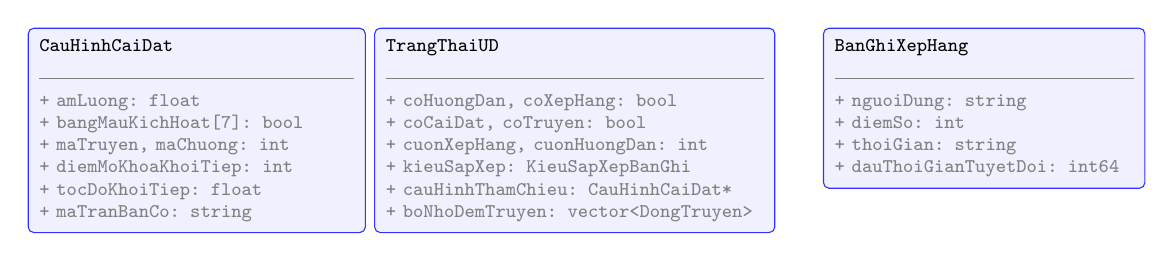
\begin{tikzpicture}[class/.style={rectangle, draw=blue!80, fill=blue!6, rounded corners=2pt, align=left, font=\scriptsize\ttfamily, inner sep=4pt}]
  \node[class, anchor=north, text width=4.0cm] (sc) at (0,0) {
    \textbf{CauHinhCaiDat}\\[2pt]
    \color{gray}\rule{\linewidth}{0.4pt}\\[2pt]
    + amLuong: float\\
    + bangMauKichHoat[7]: bool\\
    + maTruyen, maChuong: int\\
    + diemMoKhoaKhoiTiep: int\\
    + tocDoKhoiTiep: float\\
    + maTranBanCo: string
  };
  \node[class, anchor=north, text width=4.8cm] (sr) at (4.8,0) {
    \textbf{TrangThaiUD}\\[2pt]
    \color{gray}\rule{\linewidth}{0.4pt}\\[2pt]
    + coHuongDan, coXepHang: bool\\
    + coCaiDat, coTruyen: bool\\
    + cuonXepHang, cuonHuongDan: int\\
    + kieuSapXep: KieuSapXepBanGhi\\
    + cauHinhThamChieu: CauHinhCaiDat*\\
    + boNhoDemTruyen: vector<DongTruyen>
  };
  \node[class, anchor=north, text width=3.8cm] (be) at (10.0,0) {
    \textbf{BanGhiXepHang}\\[2pt]
    \color{gray}\rule{\linewidth}{0.4pt}\\[2pt]
    + nguoiDung: string\\
    + diemSo: int\\
    + thoiGian: string\\
    + dauThoiGianTuyetDoi: int64
  };
\end{tikzpicture}

% Sơ đồ 40: Seq Console
\begin{tikzpicture}[
  lhd/.style={rectangle,fill=blue!12,draw=blue!80,font=\scriptsize, inner sep=3pt,minimum width=1.8cm,align=center},
  msg/.style={-{Stealth[length=4pt]},thick},
  ret/.style={{Stealth[length=4pt]}-,thick,dashed,gray!70},
  lf/.style={draw=gray!40,dashed}
]
  \node[lhd](H1) at (0,0)    {Tệp\_Chính};
  \node[lhd](H2) at (3.2,0)  {\texttt{ChayPhanHe}\\\texttt{DieuKhien()}};
  \node[lhd](H3) at (6.4,0)  {\texttt{TangCSDL}};
  \node[lhd](H4) at (9.6,0)  {\texttt{tu}\\\texttt{SapXep}};
  \node[lhd](H5) at (12.8,0) {\texttt{HeThong}\\\texttt{VeManHinh}};
  \foreach \x in {0,3.2,6.4,9.6,12.8}{\draw[lf](\x,-0.3)--(\x,-9.0);} 
  \draw[gray!40,thick,dashed](-0.8,-4.8)--(14,-4.8);
  \node[font=\scriptsize\itshape,gray] at (-0.5,-1.0) {Luồng CHƠI};
  \node[font=\scriptsize\itshape,gray] at (-0.5,-5.5) {Luồng TRUYỆN};
  % Luồng CHƠI
  \draw[msg](0,-1.0)--(3.2,-1.0) node[above,font=\tiny,midway]{GoiHam(CauHinh)};
  \draw[msg](3.2,-1.6)--(6.4,-1.6) node[above,font=\tiny,midway]{MoCSDL+TaoBang+TaiCaiDat};
  \draw[ret](6.4,-2.1)--(3.2,-2.1) node[above,font=\tiny,midway]{CauHinh Đã Cập Nhật};
  \draw[msg](3.2,-2.5)--(9.6,-2.5) node[above,font=\tiny,midway]{TaiBangXepHang+SapXep(Diem)};
  \draw[msg](3.2,-3.0)--(12.8,-3.0) node[above,font=\tiny,midway]{VeHinhNen + VeCacNut (Vòng lặp)};
  \draw[msg](3.2,-3.5)--(6.4,-3.5) node[above,font=\tiny,midway]{LuuCaiDat(CauHinh) khi đóng Cửa Sổ};
  \draw[msg](3.2,-4.0)--(6.4,-4.0) node[above,font=\tiny,midway]{NguoiDung Nhan CHOI};
  \draw[ret](6.4,-4.4)--(0,-4.4) node[above,font=\tiny,midway]{TraVe(1) Sang Phan He Loi};

  % Luồng TRUYỆN
  \draw[msg](0,-5.5)--(3.2,-5.5) node[above,font=\tiny,midway]{GoiHam(CauHinh)};
  \draw[msg](3.2,-6.1)--(6.4,-6.1) node[above,font=\tiny,midway]{coCuaSoTruyen=True; TaiDanhSachTruyen()};
  \draw[ret](6.4,-6.6)--(3.2,-6.6) node[above,font=\tiny,midway]{BoNhoDemTruyen[]};
  \draw[msg](3.2,-7.0)--(12.8,-7.0) node[above,font=\tiny,midway]{VeCuaSoTruyen()};
  \draw[msg](3.2,-7.5)--(6.4,-7.5) node[above,font=\tiny,midway]{ChonTruyen(MaTruyen, MaChuong)};
  \node[font=\tiny,align=center] at (5.5,-8.1){\textit{CauHinh.maTruyen=M, maChuong=C,}\\ \textit{CapNhatNguongKhoi, MaTranBanCo}};
  \draw[ret](6.4,-8.6)--(0,-8.6) node[above,font=\tiny,midway]{TraVe(2) CauHinh Da Duoc Ghi};
\end{tikzpicture}

% Sơ đồ 41: Thành phần Core
\begin{tikzpicture}[
  comp/.style={rectangle,draw=blue!80,fill=blue!8,rounded corners=3pt, minimum width=3.0cm,minimum height=0.8cm,align=center,font=\small},
  ext/.style={rectangle,draw=gray!55,fill=gray!8,rounded corners=2pt, minimum width=2.6cm,minimum height=0.7cm,align=center,font=\scriptsize},
  ro/.style={rectangle,draw=green!80,fill=green!7,rounded corners=2pt, minimum width=2.6cm,minimum height=0.7cm,align=center,font=\scriptsize},
  iface/.style={-{Stealth[length=5pt]},thick},
  write/.style={-{Stealth[length=5pt]},thick,orange!80}
]
  \node[ro](main)    at (0,0)      {Tệp\_Chính};
  \node[comp](entry) at (5.0,0)    {\texttt{ChayPhanHeLoi()}\\+ Trạng thái};
  \node[ext](bgm)    at (10.0,0)   {Âm thanh Nhạc};
  \node[comp](phys)  at (5.0,-2.6) {Vòng lặp Vật lý\\(rơi/khóa/chớp)};
  \node[comp](rend)  at (0,-2.6)   {Tầng Hiển thị};
  \node[comp](inp)   at (10,-2.6)  {Bộ định tuyến Sự kiện};
  \node[comp](ogo)   at (5.0,-5.2) {\texttt{XuLyKetThucVan()}};
  \node[ext](dbw)    at (10.0,-5.2) {Ghi CSDL cục bộ};
  \node[ro](cfg)     at (5.0,-7.0) {Cấu hình (Chỉ Đọc)};

  \draw[iface](main) -- node[above=2pt, font=\tiny]{CauHinh} (entry);
  \draw[iface](entry) -- node[right=3pt, font=\tiny\color{gray}]{Luồng logic} (phys);
  \draw[iface](inp) -- node[above=2pt, font=\tiny]{Thao tác} (phys);
  \draw[iface](phys) -- node[above=2pt, font=\tiny]{Trạng thái bảng} (rend);
  \draw[iface](phys) -- node[right=3pt, font=\tiny]{Tín hiệu Dừng} (ogo);
  \draw[write](ogo) -- node[above=2pt, font=\tiny]{THÊM/CẬP NHẬT} (dbw);
  \draw[iface, dashed, green!80] (cfg.north) -- (ogo.south);
  \draw[iface, dashed, green!80] (cfg.west) -| node[pos=0.2, above, font=\tiny]{Dữ liệu cấu hình} (rend.south);
\end{tikzpicture}

% Sơ đồ 42: Trạng thái Core
\begin{tikzpicture}[
  st/.style={rectangle,draw=blue!80,fill=blue!8,rounded corners=3pt, minimum width=2.4cm,minimum height=0.8cm,align=center,font=\scriptsize},
  wasm/.style={rectangle,draw=red!80,fill=red!8,rounded corners=3pt, minimum width=2.4cm,minimum height=0.8cm,align=center,font=\scriptsize},
  arr/.style={-{Stealth[length=5pt]},thick, blue!80},
  input/.style={-{Stealth[length=5pt]},thick, dashed, gray!80},
  trans/.style={font=\tiny, align=center, inner sep=2pt, fill=white}
]
  \node[st] (init)  at (0,0)      {KHỞI TẠO};
  \node[st] (play)  at (4.5,0)    {ĐANG CHƠI};
  \node[st] (flash) at (4.5,-2.5) {CHỚP XÓA DÒNG};
  \node[st] (pause) at (9,1.5)    {TẠM DỪNG};
  \node[st] (popup) at (9,-1.5)   {HỎI THOÁT};
  \node[st] (over)  at (13.5,0)   {TRÒ CHƠI\\KẾT THÚC};
  \node[wasm](wasm) at (13.5,-2.5){TẢI LẠI TRANG};
  \draw[arr] (init) -- node[trans, above] {Vào game} (play);
  \draw[arr] (play.south) to[bend left=20] node[trans, right] {Đầy hàng} (flash.north);
  \draw[arr] (flash.west) to[bend left=20] node[trans, left] {Xong 6 nhịp} (play.south west);
  \draw[arr] (play.east) -- node[trans, above, pos=0.6] {Chạm nóc} (over.west);
  \draw[input] (play.north east) to[out=45, in=180] node[trans, above left] {Phím/Nút Dừng} (pause.west);
  \draw[input] (pause.south west) to[out=225, in=60] node[trans, below right] {Tiếp tục} (play.north east);
  \draw[input] (play.south east) to[out=-45, in=180] node[trans, below left] {Phím/Nút Thoát} (popup.west);
  \draw[input] (pause.south) -- node[trans, right] {Thoát} (popup.north);
  \draw[input] (over.north) to[bend right=30] node[trans, above] {Chơi lại (Khởi tạo)} (init.north);
  \draw[input] (popup.east) to[bend right=15] node[trans, above] {Thoát (WASM)} (wasm.west);
  \node[font=\tiny,draw=green!80,fill=green!10,rounded corners,inner sep=3pt, align=center] (ret) at (13.5,1.5) {Trở về\\Điều khiển};
  \draw[input, green!80] (over.north) -- (ret.south);
\end{tikzpicture}

% Sơ đồ 43: Sinh khối ngẫu nhiên
\begin{tikzpicture}[node distance=0.5cm, b/.style={rectangle,draw=blue!80,fill=blue!8,text width=2.8cm,align=center,font=\scriptsize,rounded corners=2pt,minimum height=0.6cm}]
  \node[b](a){Lấy Ngẫu Nhiên\\Hình Dáng Khối (1/5)};
  \node[b,right=0.6cm of a](b){50\% Xác suất:\\Lật ngang trục X};
  \node[b,right=0.6cm of b](c){Xây danh sách màu\\được kích hoạt};
  \node[b,right=0.6cm of c](d){Lấy Ngẫu Nhiên\\Chỉ Số Màu};
  \node[b,right=0.6cm of d](e){Tọa độ bắt đầu:\\Giữa nóc bảng};
  \foreach \x/\y in {a/b,b/c,c/d,d/e}{\draw[-{Stealth[length=4pt]},thick,blue!80](\x)--(\y);}
  \draw[-{Stealth[length=4pt]},thick,orange!80,bend right=20](c.south)to node[below,font=\tiny]{Lỗi: Lấy toàn bộ 6 màu}(d.south);
\end{tikzpicture}

% Sơ đồ 44: Chớp Xóa dòng
\begin{tikzpicture}[
  proc/.style={rectangle,draw=blue!80,fill=blue!8,rounded corners=2pt, minimum width=4.5cm,minimum height=0.6cm,align=center,font=\scriptsize},
  dec/.style={diamond,draw=orange!80,fill=orange!8, aspect=2.6,align=center,font=\scriptsize, inner sep=0pt},
  arr/.style={-{Stealth[length=4pt]},thick}
]
  \node[proc](p0)  at (0,0)    {\texttt{KhoaKhoi()}: Ghi ID Màu vào Bảng lưới};
  \node[proc](p1)  at (0,-1.2) {Quét hàng: Tìm các hàng đầy màu đưa vào Mảng chờ};
  \node[dec] (d0)  at (0,-2.7) {Số hàng đầy\\$> 0$?};
  \node[proc](pnc) at (5.5,-2.7){Không có: Nạp khối tiếp theo, Khởi tạo Sinh khối; KT Thua};
  \node[proc](p2)  at (0,-4.2) {Gắn Cờ Chờ Xóa; Đồng hồ Chớp = 0; Khóa luồng Khối rơi};
  \node[proc](p3)  at (0,-5.4) {Mỗi 80ms: Đồng hồ Chớp tăng; Trạng thái Chớp = Số chẵn/lẻ};
  \node[proc](p4)  at (0,-6.6) {Vẽ các hàng chờ màu trắng (Chớp sáng) hoặc tối};
  \node[dec] (d1)  at (0,-8.1) {Nhịp Chớp\\$\geq 6$?};
  \node[proc](p5)  at (5.5,-8.1){Đợi đủ 80ms tiếp theo};
  \node[proc](p6)  at (0,-9.6) {\texttt{HoanTatXoaDong()}: Điểm += $N^2$; Dịch các hàng xuống};
  \node[proc](p7)  at (0,-10.8){Gỡ Cờ Chờ Xóa; Đặt lại Đồng hồ rơi; KT Thua};

  \draw[arr](p0)--(p1); \draw[arr](p1)--(d0);
  \draw[arr](d0)--node[above, font=\tiny]{Không}(pnc);
  \draw[arr](d0)--node[left=2pt, font=\tiny]{Có}(p2);
  \draw[arr](p2)--(p3); \draw[arr](p3)--(p4); \draw[arr](p4)--(d1);
  \draw[arr](d1)--node[above, font=\tiny]{Chưa}(p5);
  \draw[arr, gray, dashed] (p5.east) -- ++(1.0,0) |- (p3.east);
  \draw[arr](d1)--node[left=2pt, font=\tiny]{Đủ}(p6); \draw[arr](p6)--(p7);
\end{tikzpicture}

% Sơ đồ 45: Thời gian chớp
\begin{tikzpicture}[every node/.style={font=\scriptsize},x=1.1cm,y=0.65cm]
  \draw[->](0,0)--(7.2,0) node[right]{Thời gian (ms)};
  \foreach \x in {0,...,6}{ \draw(\x,0.08)--(\x,-0.08) node[below]{\x$\times$80}; }
  \foreach \x/\c in {0/white!70!gray,1/gray!80,2/white!70!gray, 3/gray!80,4/white!70!gray,5/gray!80}{
    \fill[\c](\x,0.3) rectangle (\x+1,0.8);
    \draw[black](\x,0.3) rectangle (\x+1,0.8);
  }
  \node[left] at (0,0.55){Hàng bị xóa};
  \fill[red!15](0,1.0) rectangle (6,1.5);
  \draw[red!50](0,1.0) rectangle (6,1.5);
  \node[left] at (0,1.25){Chặn khối rơi};
  \draw[green!80,very thick](6,-0.4)--(6,1.7);
  \node[green!80,below] at (6,-0.5){\texttt{HoanTatXoaDong()}};
\end{tikzpicture}

% Sơ đồ 46: Tốc độ rơi
\begin{tikzpicture}[
  dec/.style={diamond,draw=orange!80,fill=orange!8, aspect=2.4,align=center,font=\scriptsize, inner sep=1pt},
  val/.style={rectangle,draw=blue!80,fill=blue!8,rounded corners=2pt, minimum width=2.0cm,minimum height=0.6cm,align=center,font=\scriptsize},
  arr/.style={-{Stealth[length=4pt]},thick},
  lbl/.style={font=\tiny, fill=white, inner sep=2pt}
]
  \node[dec](d0) at (0,0)    {Điểm\\$\geq 50$?};
  \node[dec](d1) at (0,-2.0) {Điểm\\$\geq 30$?};
  \node[dec](d2) at (0,-4.0) {Điểm\\$\geq 15$?};
  \node[dec](d3) at (0,-6.0) {Điểm\\$\geq 5$?};
  \node[val](v100) at (3.5,0)    {100\,ms};
  \node[val](v200) at (3.5,-2.0) {200\,ms};
  \node[val](v300) at (3.5,-4.0) {300\,ms};
  \node[val](v400) at (3.5,-6.0) {400\,ms};
  \node[val](v500) at (3.5,-8.0) {500\,ms (Gốc)};

  \foreach \d/\v in {d0/v100, d1/v200, d2/v300, d3/v400}{\draw[arr](\d) -- node[above, font=\tiny, pos=0.4]{Đạt}(\v);}
  \draw[arr](d0) -- node[left=3pt, font=\tiny, midway]{Chưa}(d1);
  \draw[arr](d1) -- node[left=3pt, font=\tiny, midway]{Chưa}(d2);
  \draw[arr](d2) -- node[left=3pt, font=\tiny, midway]{Chưa}(d3);
  \draw[arr](d3) |- node[left=3pt, font=\tiny, pos=0.2]{Chưa}(v500.west);
  \node[lbl, align=center] (sd_txt) at (6.5,-1.0) {Rơi Nhanh:\\$\times\frac{1}{5}$};
  \draw[arr, orange!80, dashed] (6.5,-1.8) -- (6.5,-7.5);
  \foreach \y/\v in {0/20, -2.0/40, -4.0/60, -6.0/80, -8.0/100}{ \node[font=\tiny, gray, anchor=west] at (6.8,\y){$\rightarrow$\v\,ms}; }
\end{tikzpicture}

% Sơ đồ 47: Thuật toán vuốt
\begin{tikzpicture}[
  dec/.style={diamond,draw=orange!80,fill=orange!8, aspect=2.6,align=center,font=\scriptsize, inner sep=1pt},
  act/.style={rectangle,draw=green!80,fill=green!8,rounded corners=2pt, minimum width=2.0cm,minimum height=0.6cm,align=center,font=\scriptsize},
  proc/.style={rectangle,draw=blue!80,fill=blue!8,rounded corners=2pt, minimum width=3.2cm,minimum height=0.6cm,align=center,font=\scriptsize},
  arr/.style={-{Stealth[length=4pt]},thick}
]
  \node[proc](p0) at (0,0)      {Lưu Tọa Độ Chuột (x,y) tại Vùng Lưới Chơi};
  \node[dec] (d0) at (0,-2.0)   {Chuột đè lên\\Khối đang rơi?};
  \node[proc](p1) at (0,-3.8)   {Khi Nhả Chuột: Lấy Độ Lệch dx, dy};
  \node[dec] (d1) at (-4.0,-5.8) {Vuốt trên Khối\\$|dx|>|dy|$\\$\&$ $|dx|\geq 15$?};
  \node[dec] (d2) at (4.0,-5.8)  {Vuốt vùng Nền\\$|dy|>|dx|$\\$\&$ $|dy|\geq 15$?};
  \node[act](left)  at (-5.5,-8.0) {Di Chuyển TRÁI\\nếu $dx<0$};
  \node[act](right) at (-2.5,-8.0) {Di Chuyển PHẢI\\nếu $dx>0$};
  \node[act](up)    at (2.5,-8.0)  {Xoay NGƯỢC Chiều\\nếu $dy<0$};
  \node[act](down)  at (5.5,-8.0)  {Xoay CÙNG Chiều\\nếu $dy>0$};
  \node[proc](ign)  at (0,-9.5)    {Bỏ qua thao tác (Vuốt chéo)};

  \draw[arr](p0)--node[right=5pt, font=\tiny, align=left]{Ghi nhận ToaDo\_Goc}(d0);
  \draw[arr](d0)--node[left=3pt, font=\tiny]{Có}(p1);
  \draw[arr](d0.east) to[out=0, in=0, looseness=1.8] node[right, font=\tiny]{Không}(p1.east);

  \draw[arr](p1.south) -- ++(0,-0.6) -- (-4.0,-4.4) -- (d1.north);
  \draw[arr](p1.south) -- ++(0,-0.6) -- (4.0,-4.4) -- (d2.north);
  \draw[arr](d1.south) -- ++(-1.5,-0.5) -- (left.north) node[pos=0.2, left, font=\tiny]{Đúng};
  \draw[arr](d1.south) -- ++(1.5,-0.5) -- (right.north) node[pos=0.2, right, font=\tiny]{Đúng};
  \draw[arr](d2.south) -- ++(-1.5,-0.5) -- (up.north) node[pos=0.2, left, font=\tiny]{Đúng};
  \draw[arr](d2.south) -- ++(1.5,-0.5) -- (down.north) node[pos=0.2, right, font=\tiny]{Đúng};
  \draw[arr](d1.south) -- ++(0,-2.5) -- node[above, font=\tiny]{Sai} (ign.west);
  \draw[arr](d2.south) -- ++(0,-2.5) -- node[above, font=\tiny]{Sai} (ign.east);
\end{tikzpicture}

% Sơ đồ 48: Lớp Dữ liệu Lõi
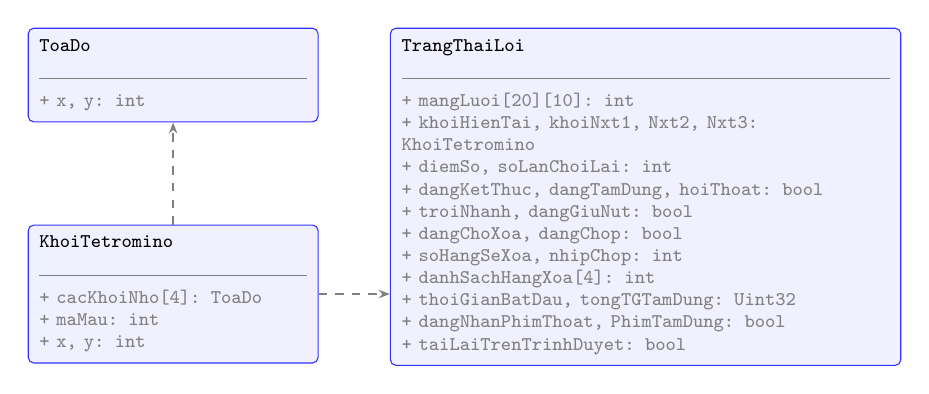
\begin{tikzpicture}[class/.style={rectangle, draw=blue!80, fill=blue!6, rounded corners=2pt, align=left, font=\scriptsize\ttfamily, inner sep=4pt}]
  \node[class, anchor=north, text width=3.4cm] (pt) at (0,0) {
    \textbf{ToaDo}\\[2pt]
    \color{gray}\rule{\linewidth}{0.4pt}\\[2pt]
    + x, y: int
  };
  \node[class, anchor=north, text width=3.4cm] (tet) at (0,-2.5) {
    \textbf{KhoiTetromino}\\[2pt]
    \color{gray}\rule{\linewidth}{0.4pt}\\[2pt]
    + cacKhoiNho[4]: ToaDo\\
    + maMau: int\\
    + x, y: int
  };
  \node[class, anchor=north, text width=6.2cm] (gs) at (6.0,0) {
    \textbf{TrangThaiLoi}\\[2pt]
    \color{gray}\rule{\linewidth}{0.4pt}\\[2pt]
    + mangLuoi[20][10]: int\\
    + khoiHienTai, khoiNxt1, Nxt2, Nxt3: KhoiTetromino\\
    + diemSo, soLanChoiLai: int\\
    + dangKetThuc, dangTamDung, hoiThoat: bool\\
    + troiNhanh, dangGiuNut: bool\\
    + dangChoXoa, dangChop: bool\\
    + soHangSeXoa, nhipChop: int\\
    + danhSachHangXoa[4]: int\\
    + thoiGianBatDau, tongTGTamDung: Uint32\\
    + dangNhanPhimThoat, PhimTamDung: bool\\
    + taiLaiTrenTrinhDuyet: bool
  };
  \draw[-{Stealth[length=4pt]}, thick, dashed, gray] (tet.north) -- (pt.south);
  \draw[-{Stealth[length=4pt]}, thick, dashed, gray] (tet.east) -- (tet.east -| gs.west);
\end{tikzpicture}

% Sơ đồ 49: DB Core
\begin{tikzpicture}[
  inmem/.style={rectangle,draw=blue!80,fill=blue!7,rounded corners=2pt, align=left,font=\scriptsize,inner sep=5pt,minimum width=3.6cm},
  owned/.style={rectangle,draw=orange!80,fill=orange!6,rounded corners=2pt, align=left,font=\scriptsize,inner sep=5pt,minimum width=3.6cm},
  write/.style={-{Stealth[length=4pt]},thick,orange!80},
  read/.style={-{Stealth[length=4pt]},dashed,gray!60},
  lbl/.style={font=\tiny,fill=white,inner sep=1.5pt}
]
  \node[inmem](gs) at (0,0) {
    \textbf{TrangThaiLoi}\ \textit{\tiny(Lưu tạm trên RAM)}\\[1pt]
    mangLuoi, diemSo\\
    khoiHienTai/KeTiep\\
    dangKetThuc, dangTamDung\\
    dangChoXoa, nhipChop\\
    thoiGianBatDau, soLanChoiLai
  };
  \node[inmem](cfg) at (0,-4.5) {
    \textbf{CauHinhCaiDat}\ \textit{\tiny(Chỉ đọc)}\\[1pt]
    amLuong, bangMauKichHoat\\
    maTruyen, maChuong\\
    diemMoKhoaKhoiTiep\\
    maTranBanCo
  };
  \node[owned](rec) at (7.5,1.2) {
    \textbf{LichSu\_Choi}\ \textit{\tiny(Thuộc quản lý Bảng điều khiển)}\\[1pt]
    \underline{ID}\ \texttt{TỰ ĐỘNG TĂNG}\\
    maNguoiDung, TGBatDau, TGKetThuc\\
    maTruyen, maChuong\\
    tongDiem, tongSoGiay\\
    tocDoTB, lanThuThu
  };
  \node[owned](stor) at (7.5,-1.5) {
    \textbf{TienDo\_NguoiDung}\ \textit{\tiny(Thuộc quản lý Bảng điều khiển)}\\[1pt]
    \underline{maNguoiDung, maTruyen, maChuong}\\
    daKichHoat, daChon\\
    tongSoLanThu, diemCaoNhat\\
    tocDoCaoNhat
  };
  \node[owned](sd) at (7.5,-4.0) {
    \textbf{DuLieu\_Chung}\ \textit{\tiny(Chỉ đọc mở khóa)}\\[1pt]
    \underline{maTruyen, maChuong}\\
    dieuKienMoKhoa\\
    nguongDiem, nguongTocDo
  };
  \draw[write](gs.east) to[out=20, in=180] node[lbl, pos=0.4]{CHÈN VÀO} (rec.west);
  \draw[write](gs.east) to[out=-20, in=180] node[lbl, pos=0.4]{CẬP NHẬT} (stor.west);
  \draw[read, blue!60](cfg.north) -- (gs.south) node[lbl, midway, align=left] {MoAmThanh\\ApDungMaTran\\SinhKhoiMoi};
  \draw[read](stor.south) -- node[lbl, left=2pt] {tra cứu} (sd.north);
  \node[font=\tiny,draw=gray!40,fill=gray!5,rounded corners,inner sep=3pt, align=center] at (3.8,-6.0) {\texttt{CoHieu\_DaLuu}:\\Đảm bảo hàm \texttt{XuLyKetThucVan()}\\chỉ chạy đúng 1 lần mỗi ván};
\end{tikzpicture}

% Sơ đồ 50: DFD Core
\begin{tikzpicture}[
  proc/.style={rectangle,draw=blue!80,fill=blue!8,rounded corners=2pt, minimum width=2.8cm,minimum height=0.6cm,align=center,font=\tiny},
  store/.style={cylinder,draw=gray!60,fill=gray!10,shape border rotate=90, minimum width=2.0cm,minimum height=0.5cm,align=center,font=\tiny, inner sep=2pt},
  extio/.style={ellipse,draw=gray!50,fill=gray!6,minimum width=2.2cm, minimum height=0.5cm,align=center,font=\tiny, inner sep=1pt},
  fl/.style={-{Stealth[length=3pt]},thick},
  dfl/.style={-{Stealth[length=3pt]},dashed,gray!80},
  lbl/.style={font=\fontsize{5}{6}\selectfont, fill=white, inner sep=1pt, align=center} 
]
  \node[extio] (ev)    at (0,5.5)     {Sự kiện SDL};
  \node[extio] (cfg2)  at (6.8,5.5)   {CauHinhCaiDat};
  \node[proc]  (route)  at (3.4,5.5)  {Bộ định tuyến Sự kiện};
  \node[proc]  (phys2)  at (3.4,3.5)  {Cập nhật Vật lý};
  \node[store] (gs2)   at (6.8,3.5)   {TrangThaiLoi};
  \node[proc]  (flash2) at (3.4,1.5)  {Hiệu ứng Chớp};
  \node[proc]  (rend3)  at (0,1.5)    {Tầng Hiển thị};
  \node[proc]  (ogo)    at (3.4,-0.5) {\texttt{XuLyKetThucVan()}};
  \node[store] (db3)   at (6.8,-0.5)  {CSDL Cục bộ};
  \node[extio] (ret2)  at (0,-0.5)    {Mã Thoát Hàm};
  
  \draw[fl] (ev) -- node[lbl, above]{hành động} (route);
  \draw[fl] (route) -- node[lbl, left, pos=0.4]{xử lý} (phys2);
  \draw[fl] (phys2) -- node[lbl, above]{Đọc/Ghi} (gs2);
  \draw[dfl] (cfg2) -- node[lbl, right]{Thông số} (gs2);
  \draw[dfl] (cfg2.west) to[out=180, in=45] node[lbl, pos=0.3]{Áp dụng} (phys2.north east);
  \draw[fl] (gs2.south) to[bend left=20] node[lbl, right]{đợi xóa} (flash2.east);
  \draw[fl] (flash2) -- node[lbl, above]{lưới bảng} (rend3);
  \draw[fl] (gs2.south) to[out=270, in=0] node[lbl, pos=0.6]{dangKetThuc} (ogo.east);
  \draw[fl] (ogo.east) -- node[lbl, above]{GHI DB} (db3.west);
  \draw[fl] (rend3.south) -- node[lbl, left]{xuất hình} (ret2.north);
\end{tikzpicture}

\end{document}